\subsubsection{Image Analysis Techniques}
	There are multiple techniques which can be applied to imagery to extract information which include detection of edges or objects and using known data to take measurements. These methods tend to compare data from neighbouring pixels to spot differences which can indicate features.
	\paragraph{Edge Detection}
	This is the application of mathematical algorithms to locate and highlight the edges of features in an image. There are multiple algorithms which can be used for edge detection including Sobel, Roberts, Canny, and fuzzy logic though all utilise the concept of comparing side by side pixel data to find "steps" from one brightness to another.
	\begin{table}[h!]
		\centering
		\caption{Table of pixel data showing an edge}
		\label{tab:edgePixels}
		\begin{tabular}{|c|c|c|c|c|c|c|}
			\hline
			5&7&6&4&152&148&149\\
			\hline
			\cellcolor[HTML]{0D0D0D}&
			\cellcolor[HTML]{121212}&
			\cellcolor[HTML]{0F0F0F}&
			\cellcolor[HTML]{0a0a0a}&
			\cellcolor[HTML]{989898}&
			\cellcolor[HTML]{949494}&
			\cellcolor[HTML]{959595}\\
			\hline
		\end{tabular}
	\end{table}\\
	Table \ref{tab:edgePixels} represents possible pixel values of an edge indicated by the large difference between 4 and 152. The applied algorithm will pick up on this discrepancy and in will be indicated on the resulting image. A common application for edge detection is text recognition such as in automatic number plate recognition (ANPR) \citep{anpr} as the process can remove unwanted background data and highlight the block shapes of the number plate.
	\begin{figure}[h!]
		\centering
		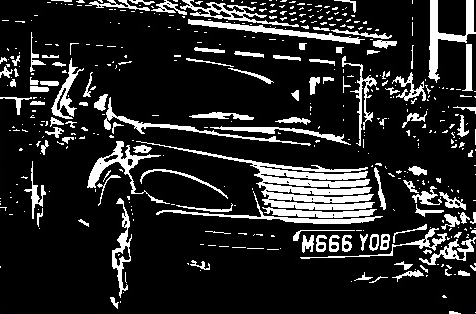
\includegraphics[width=10cm]{../images/anpr.jpg}
		\caption{Edge detection applied to an image for number plate recognition}
		\label{fig:anpr}
	\end{figure} 
	\paragraph{Object Detection}
	Much like edge detection, object detection is used to pick out features in images, the difference being that object is a more abstracted term than edge and could mean anything from faces to signs to company logos. A common technique is Binary Large OBject (BLOB) analysis which is two techniques combined into one application, this includes BLOB extraction which is used to isolate large objects in an image, dismissing small objects as noise, which is then followed by BLOB classification, assigning objects a class based on predetermined parameters.
	
	Regularly carried out after grayscaling and thresholding an image, BLOB extraction uses a grass-fire algorithm
	\paragraph{Taking Measurements}